% Template for Elsevier CRC journal article
% version 1.2 dated 09 May 2011

% This file (c) 2009-2011 Elsevier Ltd.  Modifications may be freely made,
% provided the edited file is saved under a different name

% This file contains modifications for Procedia Structural Integrity

% Changes since version 1.1
% - added "procedia" option compliant with ecrc.sty version 1.2a
%   (makes the layout approximately the same as the Word CRC template)
% - added example for generating copyright line in abstract

%-----------------------------------------------------------------------------------

%% This template uses the elsarticle.cls document class and the extension package ecrc.sty
%% For full documentation on usage of elsarticle.cls, consult the documentation "elsdoc.pdf"
%% Further resources available at http://www.elsevier.com/latex

%-----------------------------------------------------------------------------------

%%%%%%%%%%%%%%%%%%%%%%%%%%%%%%%%%%%%%%%%%%%%%%%%%%%%%%%%%%%%%%
%%%%%%%%%%%%%%%%%%%%%%%%%%%%%%%%%%%%%%%%%%%%%%%%%%%%%%%%%%%%%%
%%                                                          %%
%% Important note on usage                                  %%
%% -----------------------                                  %%
%% This file should normally be compiled with PDFLaTeX      %%
%% Using standard LaTeX should work but may produce clashes %%
%%                                                          %%
%%%%%%%%%%%%%%%%%%%%%%%%%%%%%%%%%%%%%%%%%%%%%%%%%%%%%%%%%%%%%%
%%%%%%%%%%%%%%%%%%%%%%%%%%%%%%%%%%%%%%%%%%%%%%%%%%%%%%%%%%%%%%

%% The '3p' and 'times' class options of elsarticle are used for Elsevier CRC
%% The 'procedia' option causes ecrc to approximate to the Word template
\documentclass[3p,times,procedia]{elsarticle}
\flushbottom

%% The `ecrc' package must be called to make the CRC functionality available
\usepackage{ecrc}
%\usepackage{amsmath}

\usepackage[bookmarks=false]{hyperref}
    \hypersetup{colorlinks,
      linkcolor=blue,
      citecolor=blue,
      urlcolor=blue}

%% The ecrc package defines commands needed for running heads and logos.
%% For running heads, you can set the journal name, the volume, the starting page and the authors

%% set the volume if you know. Otherwise `00'
\volume{00}

%% set the starting page if not 1
\firstpage{1}

%% Give the name of the journal
\journalname{Structural Integrity Procedia}

%% Give the author list to appear in the running head
%% Example \runauth{C.V. Radhakrishnan et al.}
\runauth{Valente et al.}

%% The choice of journal logo is determined by the \jid and \jnltitlelogo commands.
%% A user-supplied logo with the name <\jid>logo.pdf will be inserted if present.
%% e.g. if \jid{yspmi} the system will look for a file yspmilogo.pdf
%% Otherwise the content of \jnltitlelogo will be set between horizontal lines as a default logo

%% Give the abbreviation of the Journal.
\jid{prostr}

%% Give a short journal name for the dummy logo (if needed)
%\jnltitlelogo{Procedia Structural Integrity}

%% Hereafter the template follows `elsarticle'.
%% For more details see the existing template files elsarticle-template-harv.tex and elsarticle-template-num.tex.

%% Elsevier CRC generally uses a numbered reference style
%% For this, the conventions of elsarticle-template-num.tex should be followed (included below)
%% If using BibTeX, use the style file elsarticle-num.bst

%% End of ecrc-specific commands
%%%%%%%%%%%%%%%%%%%%%%%%%%%%%%%%%%%%%%%%%%%%%%%%%%%%%%%%%%%%%%%%%%%%%%%%%%

%% The amssymb package provides various useful mathematical symbols

\usepackage{amssymb}
\usepackage{siunitx}
\usepackage{physics}
%% The amsthm package provides extended theorem environments
%% \usepackage{amsthm}

%% The lineno packages adds line numbers. Start line numbering with
%% \begin{linenumbers}, end it with \end{linenumbers}. Or switch it on
%% for the whole article with \linenumbers after \end{frontmatter}.
%% \usepackage{lineno}

%% natbib.sty is loaded by default. However, natbib options can be
%% provided with \biboptions{...} command. Following options are
%% valid:

%%   round  -  round parentheses are used (default)
%%   square -  square brackets are used   [option]
%%   curly  -  curly braces are used      {option}
%%   angle  -  angle brackets are used    <option>
%%   semicolon  -  multiple citations separated by semi-colon
%%   colon  - same as semicolon, an earlier confusion
%%   comma  -  separated by comma
%%   numbers-  selects numerical citations
%%   super  -  numerical citations as superscripts
%%   sort   -  sorts multiple citations according to order in ref. list
%%   sort&compress   -  like sort, but also compresses numerical citations
%%   compress - compresses without sorting
%%
\biboptions{authoryear}

% \biboptions{}

% if you have landscape tables
\usepackage[figuresright]{rotating}
%\usepackage{harvard}
% put your own definitions here:x
%   \newcommand{\cZ}{\cal{Z}}
%   \newtheorem{def}{Definition}[section]
%   ...

% add words to TeX's hyphenation exception list
%\hyphenation{author another created financial paper re-commend-ed Post-Script}

% declarations for front matter

\begin{document}
\begin{frontmatter}

%% Title, authors and addresses

%% use the tnoteref command within \title for footnotes;
%% use the tnotetext command for the associated footnote;
%% use the fnref command within \author or \address for footnotes;
%% use the fntext command for the associated footnote;
%% use the corref command within \author for corresponding author footnotes;
%% use the cortext command for the associated footnote;
%% use the ead command for the email address,
%% and the form \ead[url] for the home page:
%%
%% \title{Title\tnoteref{label1}}
%% \tnotetext[label1]{}
%% \author{Name\corref{cor1}\fnref{label2}}
%% \ead{email address}
%% \ead[url]{home page}
%% \fntext[label2]{}
%% \cortext[cor1]{}
%% \address{Address\fnref{label3}}
%% \fntext[label3]{}

\dochead{ICSI 2023 The 5th International Conference on Structural Integrity}%

\title{Direct identification of fracture parameters of wood in mode I by digital image correlation}

%% use optional labels to link authors explicitly to addresses:
%% \author[label1,label2]{<author name>}
%% \address[label1]{<address>}
%% \address[label2]{<address>}

\author[a]{O. Cochet}
\author[b]{J. Xavier\corref{cor1}}
\author[b]{R.F. Martins}
\author[a]{R. Moutou Pitti}


\address[a]{Université Clermont Auvergne, Clermont Auvergne INP, Institut Pascal, Clermont-Ferrand, France}
\address[b]{UNIDEMI, Department of Mechanical and Industrial Engineering, NOVA School of Science and Technology, NOVA University Lisbon, 2829-516 Caparica, Portugal}

\begin{abstract}
Wood is an increasingly popular engineering material due to its potential for reducing pollution and combating global warming. Its use in construction has been recognised as a promising solution for sustainable and efficient building design. However, ensuring the safety and reliability of wooden structures requires a comprehensive understanding of the fracture mechanics of wood.
In this study, we investigate the cracking behaviour of softwood species using MMCG specimens. We aim to accurately determine crack length during fracture propagation and related fracture parameters, which is often challenging to obtain in wood. To achieve this, we employ the Arcan system to load the specimen, which has the advantage of inspecting from pure to mixed mode fracture loading to activate different failure modes. Digital Image Correlation (DIC) measures displacement and strain fields near the crack.
Our primary focus is on open I mode crack growth, and we generate force versus crack opening curves from the measurements. In addition, we use the imposed displacement compliance method to determine the strain energy release rate for opening mode.
This study highlights the importance of fracture mechanics in ensuring the safety and reliability of wooden structures. Knowledge of the fracture parameters of wood can aid in the design and development of more efficient and sustainable wooden products. Accurate determination of crack length is critical in this regard. Therefore, using digital image correlation techniques and imposed displacement compliance methods can improve our understanding of the fracture behaviour of wood and aid in the design of more reliable and efficient wooden structures.
\end{abstract}

\begin{keyword}
Digital image correlation \sep Mode I \sep Fracture parameters 
\end{keyword}
\cortext[cor1]{Corresponding author. Tel.: +351 212 948 567.}
\end{frontmatter}
%\correspondingauthor[*]{Corresponding author. Tel.: +0-000-000-0000 ; fax: +0-000-000-0000.}
\email{jmc.xavier@fct.unl.pt}

%%
%% Start line numbering here if you want
%%
% \linenumbers

%% main text

\begin{nomenclature}
\begin{deflist}[A]
\defitem{A}\defterm{radius of}
\defitem{B}\defterm{position of}
\defitem{C}\defterm{further nomenclature continues down the page inside the text box}
\end{deflist}
\end{nomenclature}

%\enlargethispage{-7mm}
\section{Introduction}\label{S:intro}

Wood is a natural resource present on all continents. In France, it represents 15 million hectares and 3.3 million hectares in Portugal. It is a natural, renewable, low energy cost, recyclable and biologically degradable material. Today, global warming is a significant concern and using wood in the construction sector would make it less polluting. It is used for many applications. It can be used as energy, in timber frames and constructions, for packaging, furniture and joinery, in the paper industry or the chemical industry, for example. In addition, the cost of wood is one of the lowest. However, the mechanical behavior of wood, and more specifically its failure properties needs to be more studied in order to design reliable structures. This lack of study may lead for instance to the sudden failure of structures during their service life, which is not acceptable. Studying the failure properties of wood is therefore crucial to guide local engineers in their choice of building materials other than concrete and steel. One of the defects of wood is its natural origin. This gives it a great source of variability in its characteristics. It is subject to weathering and, depending on the climatic conditions, it will not have the same properties. This is why it must often be used after a specific treatment.
The present document aims to study mechanical fracture of wood in mode I on silver fir specimens of type 2MCG. The proposed work consists mainly in conducting measurements carried out by kinematic field measurements obtained by the method known as image correlation or DIC. Integrating the DIC method through the MatchID software and subsequent Python-based data processing will be instrumental in attaining the desired outcomes. Two Python programs will be compared in order to verify the acuity of each method. This project consists of modelling the observed behaviour, both from the crack initiation and propagation point of view. The study will focus solely on a single wood species, and variations in wood moisture content will not be considered. The tests were carried out in a universal testing machine with a homemade Arcan fixture. This data can be used in future studies to develop computational simulations of fracture testing to determine fracture parameters from inverse methods.


%\cite{Dong201975}
\section{Methods}\label{S:method}

\subsection{Material and testing}\label{Ss:spec}

The MMCG specimen was initially developed by \citet{MoutouPitti2008}. This sample is a compromise between DCB and CTS samples to obtain different mixing rates and a stable crack propagation. The choice was made regarding to the good stability of the crack propagation. The Geometry, visible on \ref{fig:Fig5} was already tested in \citep{Odounga2018phd} works. The chosen MMCG specimens are Radial and Longitudinal surface specimens looking to the orthotropic directions of wood. 

\begin{figure}[th]
	\centering
	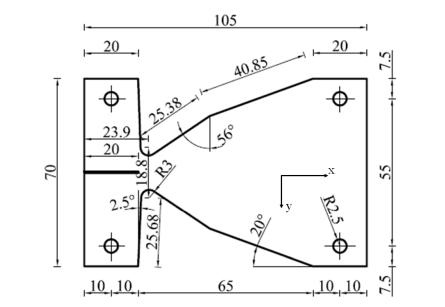
\includegraphics[scale=0.5]{Figures/fig23}
	\caption[MMCG specimen]{dimensions and geometry of Mixed Mode Crack Growth specimen}
	\label{fig:Fig5}
\end{figure}.

For the tests, the chosen European species is the silver fir, which belongs to the category of coniferous trees. This softwood species is predominantly found in the northern hemisphere, similar to pines and other aged trees. Its name originates from the white colour of its wood, and its circumference typically ranges from 50 to 80 cm. According to CIRAD data, the silver fir exhibits a density of 0.45 to 0.60, a saturation fiber point (SFP) of approximately 30\%, and a compressive strength of 41 MPa. Notably, it experiences significant tangential shrinkage at 8.7\%, while the radial shrinkage measures 4\%. Silver fir wood is commonly utilised for framing, columns, and light structures due to its strength, although it requires treatment to prevent fungal and insect attacks. However, water pockets within the tree and its susceptibility to splitting pose concerns that may limit the use of specific connectors in construction.
Wooden specimens were carefully characterised before testing by measuring weight, density, and moisture content. Before the tests, the samples were weighed, denoted as $M_H$, to determine their mass during testing. The wood density can also be derived from the sample's volume and mass. AutoCAD was employed to create a digital representation of the sample, enabling us to determine its theoretical surface, which can then be multiplied by the thickness to calculate the volume. The density of each sample can be determined by applying the formula $\rho = M/V$.
After testing, the specimens were placed in an oven set at 100 degrees until their mass, labelled as $M_C$, stabilised. Two specimens were subjected to this process for 73 hours, and various measurements were taken until a constant mass was achieved. The moisture content of the specimens can be determined using equation \ref{eq:HI}. Consequently, we possess the average mass of 29.83g, the density 431.3kg/m$^3$, and the moisture content of 10.3\%.

\begin{equation}
	HI(\%) = \frac{M_{H}-M_{0}}{M_{0}}
	\label{eq:HI}
\end{equation}

An Arcan fixture system is required to perform the  2MCG fracture tests. Indeed, this part allows the connection of the 2MCG wood specimen (Figure \ref{fig:Fig5}) to the cross-head displacement of the test frame. Figure \ref{fig:Fig6} shows the Arcan device we will use, inspired by the thesis of \citep{Odounga2018phd}.

\begin{figure}[th]
	\centering
	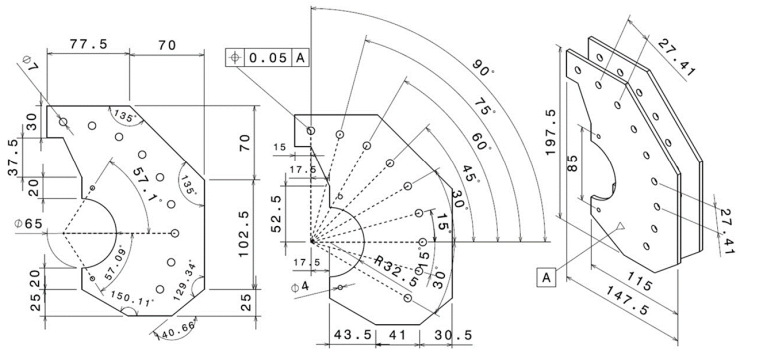
\includegraphics[scale=0.5]{Figures/fig24}
	\caption[MMCG specimen]{Size of the Arcan fastening system \citep{Odounga2018phd}.}
	\label{fig:Fig6}
\end{figure}.


The fixing holes for the wooden specimens have a diameter $\Phi= 4 mm$, and the loading holes have a diameter $\Phi = 7 mm$. These fixing holes were drilled in order to be able to load the specimen with different angular values of the angle in relation to the vertical direction in order to activate different failure modes depending on the load angle. To connect the Arcan system to the press, a piece had to be created, as shown in Figure \ref{fig:Fig7}.

\begin{figure}[th]
	\centering
	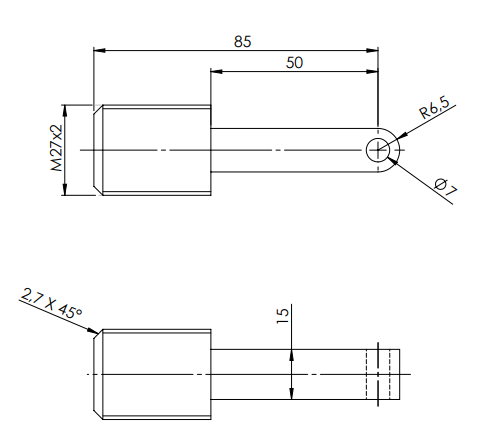
\includegraphics[scale=0.3]{Figures/fig25}
	\caption[MMCG specimen]{Bolt for connecting the press and the Arcan System.}
	\label{fig:Fig7}
\end{figure}.

This component incorporates a hole with dimensions identical to the Arcan specimen, facilitating seamless integration. Furthermore, the connector head has a diameter of 27 mm, and the thread has a pitch of 2 mm to ensure compatibility with the testing machine. The fixture was designed and assembled using SolidWorks software, and detailed technical drawings were produced for manufacturing (Figure \ref{fig:fig8}). However, before final production, a 3D printer was employed to create a prototype of the object, allowing for thorough verification and validation.

\begin{figure}[th]
	\centering
	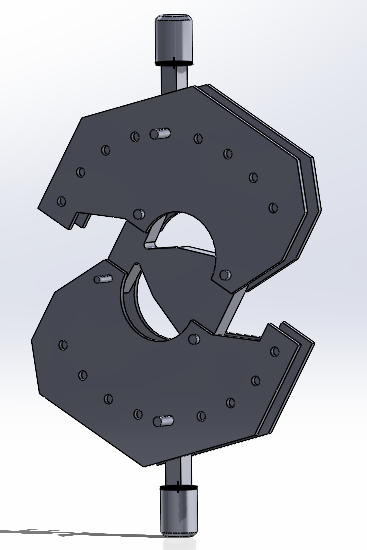
\includegraphics[scale=0.3]{Figures/fig26}
	\caption{Assembled device in Solidworks.}
	\label{fig:Fig8}
\end{figure}.

%\\\\\\\\\\\\\\\\\\\\\\\\\\\\\\\\\\\\\\\\\\\\\\\\\\\\\\\\\\

%New chapter

%\\\\\\\\\\\\\\\\\\\\\\\\\\\\\\\\\\\\\\\\\\\\\\\\\\\\\\\\\\

\subsection{Opening mode fracture loading}\label{Ss:modeIfrac}


%\\\\\\\\\\\\\\\\\\\\\\\\\\\\\\\\\\\\\\\\\\\\\\\\\\\\\\\\\\

%New chapter

%\\\\\\\\\\\\\\\\\\\\\\\\\\\\\\\\\\\\\\\\\\\\\\\\\\\\\\\\\\

\subsubsection{Compliance method}\label{Ss:complmet}

To determine the Energy release rate, compliance method was chosen. 
The formula used to calculate this energy release rate is written on \ref{eq:Energy release rate equation}:
\begin{equation}
	G_{c}= \frac{F_{c}^2}{2b} (\frac{\Delta C}{\Delta a})_{d} 	
	\label{eq:Energy release rate equation}
\end{equation}  
With : 

$G_c$ the value of energy release rate (in \si{\joule\per\square\meter})

$F_c$ the critical force which involves the crack (in \si{\newton})

b the thickness of the specimen (in \si{\milli\meter})

$\Delta C$ the compliance evolution (in $Pa^-1$)

$\Delta a$ the crack length evolution (in \si{\milli\meter})

In this work, C is determined in forced displacement, by the division of U, the imposed displacement, by F, the applied force. 


%\\\\\\\\\\\\\\\\\\\\\\\\\\\\\\\\\\\\\\\\\\\\\\\\\\\\\\\\\\

%New chapter

%\\\\\\\\\\\\\\\\\\\\\\\\\\\\\\\\\\\\\\\\\\\\\\\\\\\\\\\\\\

\subsubsection{Fracture tests}\label{Ss:fractests}

%\\\\\\\\\\\\\\\\\\\\\\\\\\\\\\\\\\\\\\\\\\\\\\\\\\\\\\\\\\

%New chapter

%\\\\\\\\\\\\\\\\\\\\\\\\\\\\\\\\\\\\\\\\\\\\\\\\\\\\\\\\\\

\subsection{Digital image correlation}\label{Ss:dic}

Digital image correlation (DIC) was developed in 1983. It is a 2D or 3D optical method that measures displacements between two images. It enables the generation of displacement and strain maps, providing valuable kinematic information. The MatchID DIC 2D software was used in this study, and Python-based scripting was coded for post-processing purposes.
The focus of this study was the evaluation of crack opening displacement and crack length variation during the fracture tests with regard to the applied load. A monotonic optical system, employing a single camera, was employed. A speckle pattern was manually applied to all specimens using white-and-black spray paint to facilitate DIC analysis. The procedure involved initially applying a thin layer of white paint using a matte spray, followed by applying black paint to create a distinctive local pattern across the region of interest (ZOI) ahead of the crack tip. Notably, care was taken during lens and camera adjustments to optimise focusing and exposure time, ensuring an appropriate spread of light intensity to prevent pixel saturation in the sensor.
In DIC processing, several steps are required:

\begin{itemize}
	\item Choose a reference image that corresponds to the first image of the test 
	\item Select multiple deformed images
	\item Define the zone of interest (ZOI) in which the crack propagates
	\item Define the  DIC setting parameters
	\item Start the DIC analysis
	\item Exploit the results
\end{itemize}

It is important to highlight the significant impact of both extrinsic and intrinsic setup parameters in digital image correlation (DIC), including subset size, subset step, strain gauge window, shape functions, and correlation criterion. These parameters play a crucial role in determining the calculated strain fields, resulting in variations in spatial resolution and resolution values that can differ by an order of magnitude or more \citep{DICguide2018}. 

In order to determine the most appropriate DIC settings, the Performance Analysis module within MatchID was employed. This tool allows for the definition of a range of options to be utilized in a design of experiments study. Parameters such as subset size, step size, and strain window can be varied systematically to enable a comprehensive comparison of the reconstruction of displacement and strain fields.

Subsequently, data from each analysis were extracted in a matrix format for each acquisition step. These data were then subjected to further analysis using Python scripting, with the aim of evaluating fracture parameters within the scope of this study.

The selected parameters for the DIC analysis play a crucial role in determining the accuracy and spatial resolution of the measured displacements and reconstructed strain fields \citep{Xavier2012207,PereiraandXavier2018}. Consequently, they are considered fundamental factors. To achieve a trade-off between spatial resolution and accuracy, a parametric analysis was conducted utilizing the Parametric Module of MatchID. The resulting DIC settings are summarized in Table~\ref{tab:MatchID_param}.

The range of values defined in this performance study, including the subset size ($f_s$), subset step, affine and quadratic displacement shape functions, the size of the strain windows, and the order of the polynomial fitting function, is defined by the table \ref{tab:MatchID_param}. It is believed that the pre-selected range of values is reflective of the permissible DIC setup parameter range.

\begin{table}[]
	\centering
	\begin{tabular}{m{.3\textwidth}m{.4\textwidth}}\toprule
		Correlation   Coefficient: & ZNCC \\
		Interpolation order: & Bicubic Splines \\ 
		Transformation order: & Quadratic \\
		Prefiltering: & Gaussian \\
		Progress history: & Spatial \\
		Subset size: & 31 \\
		Step size: & 10 \\
		Strainwindow size: & 5 \\ 
		Virtual Strain Gauge: & 71 pixel \\
		Strain interpolation: & bilinear (Q4) Lagrange polynomials\\
		Strain Convention: & Green-Lagrange \\\bottomrule
	\end{tabular}
	\caption{DIC setting parameters used in the MatchID software for the analyses.}
	\label{tab:MatchID_param}
\end{table}


%\\\\\\\\\\\\\\\\\\\\\\\\\\\\\\\\\\\\\\\\\\\\\\\\\\\\\\\\\\

%New chapter

%\\\\\\\\\\\\\\\\\\\\\\\\\\\\\\\\\\\\\\\\\\\\\\\\\\\\\\\\\\

\subsubsection{Optical set-up and settings}\label{Ss:optical}

An Allied Vision Manta 505B 2/3'' camera coupled to an Opto Engineering TC 23 36 telecentric lens were used for image formation and acquisition. The camera is equipped with Charge-Coupled Device (CCD) sensor with pixel resolution of 2452 (H) $\times$ 2056 (V) (5MP) and sensor size of 2/3''. The monovision camera-lense optical system was fixed on a tripod and its spatial position oriented with regard to the target surface of interest. The telecentric lens has a magnification factor of \num{0.243}$\times$, allowed to image a field of view, in the object space, of 36.2$\times$27.1 \si{\milli\meter\squared}. The front of the lens was positioned at a working distance of 103.5 \si{\milli\meter} with an aperture of $f$/8, yielding a field of depth of 11 \si{\milli\meter}.

A high power adjustable ring light was used to illuminate the region of interest. A monochromatic version corresponding to a green wavelength of \num{525} \si{\nano\meter} was used from which the highest spectral response of the camera sensor will be expected.

All the specimens were painted to obtain a speckle pattern suitable for image correlation. A thin layer of white paint was firstly added using a mate spray, followed by a diffuse distribution of black paint to create a unique local pattern across the region of interest at the crack tip (Figure~\ref{fig:Fig17}).

\begin{figure}[t]
	\centering
	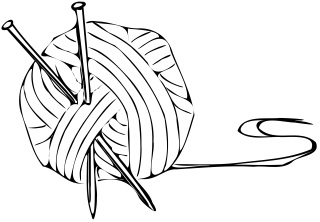
\includegraphics[width=.9\textwidth]{Figures/example}
	\caption{(a) Speckle pattern typically obtained for DIC measurements (2452 $\times$ 2056
		pixels\textsuperscript{2}); (b) Histogram
		of the
		speckle image
		(256
		gray levels, 8 bits camera).}
	\label{fig:Fig17}
\end{figure}

The DIC setting parameters can have a significant influence on the kinematic fields obtained by image correlation (\textit{e.g.} subset size, subset step, \ldots) and numerical differentiation (\textit{e.g.} strain windows size) algorithms \cite{Pereira2018566}. These settings represent fundamental parameters since they will define the spatial resolution and accuracy associated to the DIC measurements, both in displacement and strain fields.  Therefore, a parametric study was carried out to justify the DIC setting for the current
application, in a balance between resolution and spatial resolution. This study was carried ot in the Parametric Module of MatchID 2D software.
\begin{table}[]
	\centering
	\begin{tabular}{c c}
		\hline
		Correlation   Coefficient: & ZNSSD \\ 
		Interpolation order: & Bicubic Splines \\ 
		Transformation order: & Affine \\
		Subset size: & 21 \\
		Step size: & 5 \\
		Maximum rigid body estimation: & 100 \\ 
		Strain Estimation(\%): & 5 \\ 
		Precision: & 0.001 \\ 
		Maximum iterations: & 20 \\ 
		Noise handling: & Gaussian \\ 
		Kernel Size: & 5 \\ 
		History: & Spatial \\ 
		Strainwindow size: & 7 \\ 
		Tolerance on number of points: & 0 \\ 
		Strain interpolation: & Q4 \\ 
		Strain Convention: & Green-Lagrange \\ \hline
	\end{tabular}
	\caption{MatchID parameters used}
	\label{tab:MatchID_param}
\end{table}
\ref{tab:MatchID_param} defines the range of values defined in this performance analysis which includes the subset size ($f_s$), subset step, affine and quadratic displacement shape functions, the strain windows size and the order of the polynomial fitting function. The pre-selected range of values are deemed to be representative of the range of acceptable DIC setting parameters. For instance, The lower pixel boundary is constrained by aliasing effects, which is a function of the speckle size on the imaged pattern. The subset size defines the target matching pattern used in the correlation algorithm. A rule of thumb will be three contrasted speckles per subset. The average speckle size was determined as 4.5 pixels. Therefore, the minimum subset step was set to 15 pixels. The upper pixel limit can be problem-dependent, taking into account the deformation gradients expected within the region of interest, in a balance between spatial resolution and resolution. As a guideline, larger subsets improves the resolution but decreases spatial resolution. Parameters such as the subset step ($f_p$) (distance between centroids of adjacent subsets, units: pixels) and the strain window $\varepsilon_w$ (number of subsets central points used to define a mesh of data points over which a piecewise polynomial fitting will be applied, using least-square regression, for strain reconstruction) will define a strain spatial resolution ($\Delta \varepsilon$) and virtual strain gauge (VSG), respectively, according to the following relationships \cite{Lava2013576,Pereira2018566}: $\Delta \varepsilon = (\varepsilon_w-1)f_p + f_s$ and $\mbox{VSG} = (\varepsilon_w-1)f_p + 1$ (unit: pixel). For convenience, these parameters can be converted to physical units in the object space (\textit{e.g.} mm), by simple multiplication by the conversion factor of the optical imaging system. All these external DIC parameters, therefore, must be carefully selected in the current study.


Here, all the matrix, composed of the subsets from the Zone of Interest are changed by the different steps shown overhead. All the subsets are considered four by four and the displacement from one compared to it neighbor are computed. Then average and maximum values are obtained for each subset of the ZOI and put into a matrix (named K overhead). By using the $a_{0}$ data and looking to an alpha parameter, the programm compute the best shape of a(t). Alpha parameter allow to avoid the image noise but is close enough to give precise a(t) values.
This method was the one used by \cite{Reference14} on MatLab, and have already proved obtention of good results.

%\\\\\\\\\\\\\\\\\\\\\\\\\\\\\\\\\\\\\\\\\\\\\\\\\\\\\\\\\\

%New chapter

%\\\\\\\\\\\\\\\\\\\\\\\\\\\\\\\\\\\\\\\\\\\\\\\\\\\\\\\\\\


As shown in the code, the dimensions of the matrix take in account the number of stages, so the number of images. Indeed, the interest of the CTOD is to be followed at each stage. 

Then, a loop is created, allowing to put information into others vectors

Another one is also created to compared to mode II values. In the current case, the mode II can be approximate around zero, because it is a mode I test. Then all the values are obtained, for each COD pair until $ud_lim$ which is in this case equal to 10. By looking to this different curves, the chosen COD pair is chosen and a curve is plot looking to the values for this parameter chosen by the user. 

\begin{figure}[h]
	\centering
	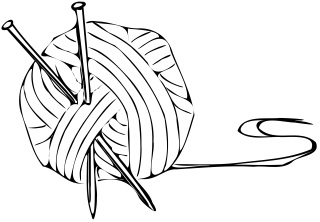
\includegraphics[scale=0.7]{Figures/example}
	\caption[Subset choice and pair of subset around]{Pair of subset around the $a_{0}$ subset chosen}
	\label{fig:subest_chosen}
\end{figure}

Finally, the way to obtain CTOD, need also a well $a_{0}$ choice. Indeed, the chosen subset as presented on \ref{fig:subest_chosen}, will be determinant. Considering the image as a matrix composed of subset, the chosen subset as a position given by his m row and n column. To determinate the opening, it is necessary to have a look on the subsets in the same n column but at a different line. Indeed, the chosen subset will be the first one affected by the crack, that means, that information on the subset will not have importance anymore. While, looking to subset up and down allow to follow the displacement of the crack tip and measure it. The fact is to determine which pair of subsets is the best. The ones at the row n-1 and n+1, but maybe these ones will be on the crack at a given stage, and will lose all the necessary information. That is why, an important choice must be done. Here, COD pair was fixed equal to two. So the subset displacement analysed is the one of the pair of subset 2 on \ref{fig:subest_chosen}. Finally, by looking to these displacements, it is possible to obtain the value of the crack opening at each stages.

%\\\\\\\\\\\\\\\\\\\\\\\\\\\\\\\\\\\\\\\\\\\\\\\\\\\\\\\\\\

%New chapter

%\\\\\\\\\\\\\\\\\\\\\\\\\\\\\\\\\\\\\\\\\\\\\\\\\\\\\\\\\\

\section{Results}\label{S:res}
\subsection{Maximum Load}\label{S:pdcurves}

The first results, obtained with the servohydraulic press were, as presented in \ref{fig:Res_Pmax}, the necessary loads to involve a propagation of the crack in all the ZOI and sometimes until the entire destruction of the specimen.

\begin{figure}[th]
	\centering
	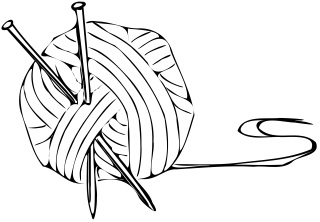
\includegraphics[width=\textwidth]{Figures/example}
	\caption[Maximal load reach for each specimen]{Maximal load reach for each specimen compared to the Moisture Content of the specimens}
	\label{fig:Res_Pmax}
\end{figure}

As expected, Padouck specimens need a higher load to involve the final crack. It was obvious, that the denser material is more difficult to destroy than the lower one.

%\\\\\\\\\\\\\\\\\\\\\\\\\\\\\\\\\\\\\\\\\\\\\\\\\\\\\\\\\\

%New chapter

%\\\\\\\\\\\\\\\\\\\\\\\\\\\\\\\\\\\\\\\\\\\\\\\\\\\\\\\\\\


\section{Discussion}\label{S:dis}

This work is really interesting compared to previous ones. In every works the MC increase phenomenon decrease the Resistance of the material. The G and the $\sigma$ were obtained on European species and this trend was confirmed. But since the beginning of tests on Tropical species, others behavior are found. \cite{Reference7} has proved by his work, that the results, regarding to the mode and the load angle applied, for Iroko, Okoume and Padouck, are similar to European ones. But no proof were already done concerning the behavior of this species to MC effect. This species from Gabon are submitted to higher temperature and relative humidity around 80\%. And looking to work as \cite{Kif1998} and \cite{Ang2017}, the density of Scots Pine and Douglas, can be compared to Okoume specimens, and then the results from these specimens can be discussed. It appears that the early wood more saturated in water than the lately one involves a decrease of the $\sigma$. A similar trend is shown on Douglas Fir regarding two MC values, 9\% and 18\%. The fact is that the Okoume species do not have this trend and is stable.



%\\\\\\\\\\\\\\\\\\\\\\\\\\\\\\\\\\\\\\\\\\\\\\\\\\\\\\\\\\

%New chapter

%\\\\\\\\\\\\\\\\\\\\\\\\\\\\\\\\\\\\\\\\\\\\\\\\\\\\\\\\\\

\section{Conclusions}\label{S:con}

In conclusion, this study aimed to investigate the fracture parameters of silver fir, a type of softwood species. The Arcan fixture was utilised to apply mode I fracture loading. Wooden specimens were specifically manufactured along the RL propagation planes. Digital image correlation (DIC) with MatchID software was employed to analyse the deformation patterns, and a Python code was developed for subsequent data processing to obtain fracture parameters, including crack tip opening displacement and crack length evaluation during the fracture tests.
The experiments focused on open mode (mode I) tests conducted on MMCG specimens. The critical energy release rate for each specimen was calculated using the compliance method. Comparative analysis of the average $G_{max}$ values with those of other temperate species revealed significant similarities, providing valuable insights into the fracture behaviour of silver fir.
Moving forward, the geometry of the MMCG specimen, the Arcan system, and the developed Python code can be readily applied to future tests. It would be particularly intriguing to conduct tests in both mode I and mixed mode I+II using different wood species whilst also considering variations in humidity and temperature levels. Such comprehensive investigations would enhance our understanding of wood behaviour. However, it is important to acknowledge that due to the intricate nature of wood's behaviour, developing empirical models may be challenging, and each tested sample will likely exhibit unique characteristics. Therefore, numerous experiments are necessary to explore the complexities of this biological material.

%\begin{table}[h]
%\caption{An example of a table.}
%\begin{tabular*}{\hsize}{@{\extracolsep{\fill}}lll@{}}
%\toprule
%An example of a column heading & Column A ({\it{t}}) & Column B ({\it{t}})\\
%\colrule
%And an entry &   1 &  2\\
%And another entry  & 3 &  4\\
%And another entry &  5 &  6\\
%\botrule
%\end{tabular*}
%\end{table}

%\enlargethispage{12pt}

%Reference generation by using bibliography style commands for LaTeX template only.
%
%The author may use ``elsarticle-harv.bst'' as per the style required in document. The sample bib file could be referred.
%If the author may using bibstyle for providing references author must comment the bibliography section in TeX file, Bibtex will generate the reference automatically.
%
%If the author may not able to view the references in output same could be done by copying the bibliography section from ``filename.bbl'' file and paste in TeX file.


\subsection{General guidelines for the preparation of your text}
Avoid hyphenation at the end of a line. Symbols denoting vectors and matrices should be indicated in bold type. Scalar variable names should normally be expressed using italics. Weights and measures should be expressed in SI units. All non-standard abbreviations or symbols must be defined when first mentioned, or a glossary provided.

%\begin{figure}[t]\vspace*{4pt}
%%\centerline{\includegraphics{fx1}\hspace*{5mm}\includegraphics{fx1}}
%\centerline{\includegraphics{gr1}}
%\caption{(a) first picture; (b) second picture.}
%\end{figure}

%\begin{equation}
%\begin{array}{lcl}
%\displaystyle X_r &=& \displaystyle\dot{Q}^{''}_{rad}\left/\left(\dot{Q}^{''}_{rad} + \dot{Q}^{''}_{conv}\right)\right.\\[6pt]
%\displaystyle \rho &=& \displaystyle\frac{\vec{E}}{J_c(T={\rm const.})\cdot\left(P\cdot\left(\displaystyle\frac{\vec{E}}{E_c}\right)^m+(1-P)\right)}
%\end{array}
%\end{equation}

\section*{Acknowledgements}

This research was funded by the project UIDB/00667/2020 (UNIDEMI) supported
by Fundação para a Ciência e a Tecnologia (FCT-MCTES), the Portuguese
national funding agency for science, research and technology.

%% The Appendices part is started with the command \appendix;
%% appendix sections are then done as normal sections
%% \appendix

%% \section{}
%% \label{}

%\appendix
%\section{An example appendix}
%Authors including an appendix section should do so before References section. Multiple appendices should all have headings in the style used above. They will automatically be ordered A, B, C etc.
%
%\subsection{Example of a sub-heading within an appendix}
%There is also the option to include a subheading within the Appendix if you wish.

%% References
%%
%% Following citation commands can be used in the body text:
%% Usage of \cite is as follows:
%%   \cite{key}         ==>>  [#]
%%   \cite[chap. 2]{key} ==>> [#, chap. 2]
%%

%The citation must be used in following style: \cite{article-minimal} \cite{article-full} \cite{article-crossref} \cite{whole-journal}.
%% References with BibTeX database:

\bibliography{biblio}
\bibliographystyle{elsarticle-harv}

%% Authors are advised to use a BibTeX database file for their reference list.
%% The provided style file elsarticle-num.bst formats references in the required Procedia style

%%% For references without a BibTeX database:
%
% \begin{thebibliography}{}
%
%%% \bibitem must have the following form:
%%%   \bibitem{key}...
%%%
%
%\bibitem[Clark et al.(1962)]{clark}Clark, T., Woodley, R.,
%De Halas, D., 1962. Gas-Graphite Systems, in ``{\it
%Nuclear
%Graphite}''.
%In: Nightingale, R. (Ed.). Academic Press, New York, pp.
%387.
%
%\bibitem[Deal and Grove(2009) ]{Deal}Deal, B., Grove, A.,
%1965. General Relationship for the Thermal Oxidation of
%Silicon. Journal of Applied Physics 36, 37--70.
%
%\bibitem[Deep(2009)]{Deep}Deep-Burn Project: Annual Report
%for 2009, Idaho National Laboratory, Sept. 2009.
%
%\bibitem[Fachinger(2004)]{Fachinger2004}Fachinger, J., den
%Exter, M., Grambow, B., Holgerson, S., Landesmann, C.,
%Titov, M., Podruhzina, T., 2004. ``Behavior of spent HTR
%fuel elements in aquatic phases of repository host rock
%formations,'' 2nd International Topical Meeting on High
%Temperature Reactor Technology. Beijing, China, paper
%\#B08.
%
%\bibitem[Fachinger(2006)]{Fachinger2006}Fachinger, J.,
%2006. Behavior of HTR Fuel Elements in Aquatic Phases of
%Repository Host Rock Formations. Nuclear Engineering \&
%Design 236,     54.
%
%
% \end{thebibliography}
%
%\clearpage

%%%% This page is for instructions only, once the article is finalize please omit the below text before creating the final PDF
%\normalMode
%
%\section*{Instructions to Authors for LaTeX template:}
%
%\section{ZIP mode for LaTeX template:}
%
%The zip package is created as per the guide lines present on the URL http://www.elsevier.com/author-schemas/ preparing-crc-journal-articles-with-latex for creating the LaTeX zip file of Procedia LaTeX template.  The zip generally contains the following files:
%\begin{Itemize}[]\leftskip-17.7pt\labelsep3.3pt
%\item ecrc.sty
%\item  elsarticle.cls
%\item elsdoc.pdf
%\item .bst file
%\item Manuscript templates for use with these bibliographic styles
%\item  Generic and journal specific logos, etc.
%\end{Itemize}
%
%The LaTeX package is the main LaTeX template. All LaTeX support files are required for LaTeX pdf generation from the LaTeX template package.
%
%{\bf Reference style .bst file used for collaboration support:} In the LaTeX template packages of all Procedia titles a new ``.bst'' file is used which supports collaborations downloaded from the path http://www.elsevier.com/author-schemas/the-elsarticle-latex-document-class

\end{document}

%%
%% End of file `prostr-template.tex'.
